% !TEX spellckeck=en_GB

\section{Neural networks}\label{sec:ANN}

While the basis for the modern neural network was laid more than a hundred years ago in the late 1800's what we think of as neural networks in modern terms was proposed by \citet{McCulloch1943}. They described a computational structure analogous to a human neuron. Dubbed an Artificial Neural Network (ANN) it takes input from multiple sources, weights that input and produces an output if the signal from the weighted input is strong enough. A proper derivation will follow but for the moment we explore this simple intuition. These artificial neurons are ordered in layers, each successively passing information forward to a final output. The output can be categorical or real-valued in nature. A simple illustration of two neurons in one layer is provided in figure \ref{fig:ann_illustration}


\tikzset{every picture/.style={line width=0.75pt}} %set default line width to 0.75pt        


\begin{figure}[h]
\centering
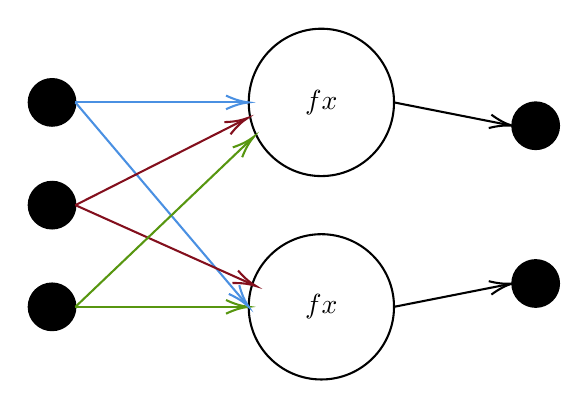
\begin{tikzpicture}[x=0.75pt,y=0.75pt,yscale=-1,xscale=1]
%uncomment if require: \path (0,300); %set diagram left start at 0, and has height of 300

%Flowchart: Connector [id:dp526297050187353] 
\draw   (285,88.5) .. controls (285,68.89) and (300.67,53) .. (320,53) .. controls (339.33,53) and (355,68.89) .. (355,88.5) .. controls (355,108.11) and (339.33,124) .. (320,124) .. controls (300.67,124) and (285,108.11) .. (285,88.5) -- cycle ;
%Flowchart: Connector [id:dp5646385359122916] 
\draw   (285,187) .. controls (285,167.67) and (300.67,152) .. (320,152) .. controls (339.33,152) and (355,167.67) .. (355,187) .. controls (355,206.33) and (339.33,222) .. (320,222) .. controls (300.67,222) and (285,206.33) .. (285,187) -- cycle ;
%Flowchart: Connector [id:dp3104075761318521] 
\draw  [fill={rgb, 255:red, 0; green, 0; blue, 0 }  ,fill opacity=1 ] (179,88.5) .. controls (179,82.29) and (184.04,77.25) .. (190.25,77.25) .. controls (196.46,77.25) and (201.5,82.29) .. (201.5,88.5) .. controls (201.5,94.71) and (196.46,99.75) .. (190.25,99.75) .. controls (184.04,99.75) and (179,94.71) .. (179,88.5) -- cycle ;
%Flowchart: Connector [id:dp15106578289314898] 
\draw  [fill={rgb, 255:red, 0; green, 0; blue, 0 }  ,fill opacity=1 ] (179,187) .. controls (179,180.79) and (184.04,175.75) .. (190.25,175.75) .. controls (196.46,175.75) and (201.5,180.79) .. (201.5,187) .. controls (201.5,193.21) and (196.46,198.25) .. (190.25,198.25) .. controls (184.04,198.25) and (179,193.21) .. (179,187) -- cycle ;
%Flowchart: Connector [id:dp06829960407828417] 
\draw  [fill={rgb, 255:red, 0; green, 0; blue, 0 }  ,fill opacity=1 ] (179,138) .. controls (179,131.79) and (184.04,126.75) .. (190.25,126.75) .. controls (196.46,126.75) and (201.5,131.79) .. (201.5,138) .. controls (201.5,144.21) and (196.46,149.25) .. (190.25,149.25) .. controls (184.04,149.25) and (179,144.21) .. (179,138) -- cycle ;
%Straight Lines [id:da16938395812882923] 
\draw [color={rgb, 255:red, 74; green, 144; blue, 226 }  ,draw opacity=1 ]   (201.5,88.5) -- (283,88.5) ;
\draw [shift={(285,88.5)}, rotate = 180] [color={rgb, 255:red, 74; green, 144; blue, 226 }  ,draw opacity=1 ][line width=0.75]    (10.93,-3.29) .. controls (6.95,-1.4) and (3.31,-0.3) .. (0,0) .. controls (3.31,0.3) and (6.95,1.4) .. (10.93,3.29)   ;

%Straight Lines [id:da6971592528694486] 
\draw [color={rgb, 255:red, 87; green, 150; blue, 16 }  ,draw opacity=1 ][fill={rgb, 255:red, 0; green, 0; blue, 0 }  ,fill opacity=1 ]   (201.5,187) -- (283,187) ;
\draw [shift={(285,187)}, rotate = 180] [color={rgb, 255:red, 87; green, 150; blue, 16 }  ,draw opacity=1 ][line width=0.75]    (10.93,-3.29) .. controls (6.95,-1.4) and (3.31,-0.3) .. (0,0) .. controls (3.31,0.3) and (6.95,1.4) .. (10.93,3.29)   ;

%Straight Lines [id:da7906184612815319] 
\draw [color={rgb, 255:red, 74; green, 144; blue, 226 }  ,draw opacity=1 ]   (201.5,88.5) -- (283.71,185.47) ;
\draw [shift={(285,187)}, rotate = 229.71] [color={rgb, 255:red, 74; green, 144; blue, 226 }  ,draw opacity=1 ][line width=0.75]    (10.93,-3.29) .. controls (6.95,-1.4) and (3.31,-0.3) .. (0,0) .. controls (3.31,0.3) and (6.95,1.4) .. (10.93,3.29)   ;

%Straight Lines [id:da1362874028964085] 
\draw [color={rgb, 255:red, 131; green, 15; blue, 29 }  ,draw opacity=1 ][fill={rgb, 255:red, 0; green, 0; blue, 0 }  ,fill opacity=1 ]   (201.5,138) -- (282.72,96.9) ;
\draw [shift={(284.5,96)}, rotate = 513.1600000000001] [color={rgb, 255:red, 131; green, 15; blue, 29 }  ,draw opacity=1 ][line width=0.75]    (10.93,-3.29) .. controls (6.95,-1.4) and (3.31,-0.3) .. (0,0) .. controls (3.31,0.3) and (6.95,1.4) .. (10.93,3.29)   ;

%Straight Lines [id:da569846296368284] 
\draw [color={rgb, 255:red, 131; green, 15; blue, 29 }  ,draw opacity=1 ][fill={rgb, 255:red, 0; green, 0; blue, 0 }  ,fill opacity=1 ]   (201.5,138) -- (286.67,176.18) ;
\draw [shift={(288.5,177)}, rotate = 204.15] [color={rgb, 255:red, 131; green, 15; blue, 29 }  ,draw opacity=1 ][line width=0.75]    (10.93,-3.29) .. controls (6.95,-1.4) and (3.31,-0.3) .. (0,0) .. controls (3.31,0.3) and (6.95,1.4) .. (10.93,3.29)   ;

%Straight Lines [id:da6518887295694358] 
\draw [color={rgb, 255:red, 87; green, 150; blue, 16 }  ,draw opacity=1 ][fill={rgb, 255:red, 0; green, 0; blue, 0 }  ,fill opacity=1 ]   (201.5,187) -- (286.05,106.38) ;
\draw [shift={(287.5,105)}, rotate = 496.36] [color={rgb, 255:red, 87; green, 150; blue, 16 }  ,draw opacity=1 ][line width=0.75]    (10.93,-3.29) .. controls (6.95,-1.4) and (3.31,-0.3) .. (0,0) .. controls (3.31,0.3) and (6.95,1.4) .. (10.93,3.29)   ;

%Flowchart: Connector [id:dp5234386771770392] 
\draw  [fill={rgb, 255:red, 0; green, 0; blue, 0 }  ,fill opacity=1 ] (412,99.75) .. controls (412,93.54) and (417.04,88.5) .. (423.25,88.5) .. controls (429.46,88.5) and (434.5,93.54) .. (434.5,99.75) .. controls (434.5,105.96) and (429.46,111) .. (423.25,111) .. controls (417.04,111) and (412,105.96) .. (412,99.75) -- cycle ;
%Flowchart: Connector [id:dp4431827599012259] 
\draw  [fill={rgb, 255:red, 0; green, 0; blue, 0 }  ,fill opacity=1 ] (412,175.75) .. controls (412,169.54) and (417.04,164.5) .. (423.25,164.5) .. controls (429.46,164.5) and (434.5,169.54) .. (434.5,175.75) .. controls (434.5,181.96) and (429.46,187) .. (423.25,187) .. controls (417.04,187) and (412,181.96) .. (412,175.75) -- cycle ;
%Straight Lines [id:da8359806786193378] 
\draw    (355,88.5) -- (410.04,99.36) ;
\draw [shift={(412,99.75)}, rotate = 191.16] [color={rgb, 255:red, 0; green, 0; blue, 0 }  ][line width=0.75]    (10.93,-3.29) .. controls (6.95,-1.4) and (3.31,-0.3) .. (0,0) .. controls (3.31,0.3) and (6.95,1.4) .. (10.93,3.29)   ;

%Straight Lines [id:da2250239797689928] 
\draw    (355,187) -- (410.04,176.14) ;
\draw [shift={(412,175.75)}, rotate = 528.8399999999999] [color={rgb, 255:red, 0; green, 0; blue, 0 }  ][line width=0.75]    (10.93,-3.29) .. controls (6.95,-1.4) and (3.31,-0.3) .. (0,0) .. controls (3.31,0.3) and (6.95,1.4) .. (10.93,3.29)   ;


% Text Node
\draw (320,88.5) node   {$fx$};
% Text Node
\draw (320,187) node   {$fx$};
\end{tikzpicture}
\caption{An illustration of the graph constructed by two artificial neurons with three input nodes. Colored lines illustrate that  each of the input nodes are connected to each of the neurons in a manner we denote as fully-connected.}\label{fig:ann_illustration}
\end{figure}


\noindent The ANN produces an output by a "forward pass". If we let the input to an ANN be $x \in \R^N$, and letting the matrix $W \in \R^{N \times D}$ be a representation of the weight matrix forming the connections between the input and the artificial neurons. Lastly we define the activation function $a(x)$ as a monotonic, once differentiable, function on $\R^1$. The function $a(x)$ determines the complexity of the neural network together with the number of neurons per layer and number of layers. For any complex task the activation takes a non-linear form which allows for the representation of more complex problems. A layer in a network implements what we will call a forward pass as defined in function \ref{eq:fwd}.

\begin{equation}\label{eq:fwd}
	\hat{y} = a(\inner{x}{W})_D
\end{equation}

\noindent In equation \ref{eq:fwd} the subscript denotes that the function is applied element-wise and we denote the matrix inner product in bra-ket notation with $\inner{\cdot}{\cdot}$. Each node is additionally associated with a bias node ensuring that even zeroed-neurons can encode information. Let the bias for the layer be given as $b \in \R^D$ in keeping with the notation above. Equation \ref{eq:fwd} then becomes:

\begin{equation}\label{eq:fwd_b}
	\hat{y} = a(\inner{x}{W})_D + b
\end{equation}

\noindent As a tie to more traditional methods we note that if we only have one layer and a linear activation $a(x) = x$ the ANN becomes the formulation for a linear regression model. In our model the variables that need to be fit are the elements of $W$ that we denote $\wij$. While one ordinarily solves optimization problem for the linear regression model by matrix inversion, we re-frame the problem in more general terms here to prime the discussion of the optimization of multiple layers and a non linear activation function. The objective of the ANN is formulated in a "loss function", which encodes the difference between the intended and achieved output. The loss will be denoted as $\mathcal{L}(y, \hat{y}, W)$. Based on whether the output is described by real values, or a set of probabilities this function, $\loss$, takes on the familiar form of the Mean Squared Error or in the event that we want to estimate the likelihood of the output under the data; the binary cross-entropy. We will also explore these functions in some detail later. The ansatz for our optimization procedure is given in the well known form of a gradient descent procedure in equation \ref{eq:gd}

\begin{equation}\label{eq:gd}
	\wij \leftarrow -\eta \frac{\partial \loss}{\partial \wij} + \wij 
\end{equation}

\subsection{Backpropagation}\label{sec:backpropagation}

In the vernacular of the machine learning literature the aim of the optimization procedure is to "train" the model to perform better on the regression, reconstruction or classification task at hand. Training the model requires the computation of the total derivative in equation \ref{eq:gd}. This is also where the biological metaphor breaks down, as the brain is almost certainly not employing an algorithm so crude as to be formulated by gradient descent. Backpropagation, or automatic differentiation, first described by \citet{Linnainmaa1976}, is a method of computing the partial derivatives required to go from the gradient of the loss w.r.t the output of the ANN to the gradient w.r.t the individual neuron weights in the layers of the ANN. The algorithm begins with computing the total loss, here exemplified with the squared error function, in equation \ref{eq:tot_err}

\begin{equation}\label{eq:tot_err}
	E = \mathcal{L}(y, \hat{y}, W) = \frac{1}{2}\sum_n \sum_j (y_{nj} - \hat{y}_{nj})^2
\end{equation}

\noindent The factor one half is included for practical reasons to cancel the exponent under differentiation. As the gradient is multiplied by an arbitrary learning rate $\eta$ this is ineffectual on the training itself. The sums define an iteration over the number of samples, and number of output dimensions respectively. Taking the derivative of \ref{eq:tot_err} w.r.t the output, $\hat{y}$, we get 

\begin{equation}\label{eq:err_grad}
	\frac{\partial E}{\partial \hat{y}_{j}} = \hat{y}_{j}^M -  y_{j} 
\end{equation}

\noindent Recall now that for an ANN with M layers the output fed to the activation function is 
\begin{equation}\label{eq:fwd_multi}
	x_{j}^M = \inner{a^{M-1}}{W^M} + b_j
\end{equation}

\noindent Where the superscript in the inner product denote the output of the second-to-last layer and the weight matrix being the last in the layers. The vector $x_{j}$ is then fed to the activation to compute the output 

\begin{equation}
\hat{y}_{j}^M = a(x_{j}^M) 
\end{equation}

\noindent  The activation function was classically the sigmoid (logistic) function but during the last decade the machine learning community has shifted to largely using the rectified linear unit (ReLU) as activation. Especially after the success of \citet{Krizhevsky2012} with AlexNET in image classification. Depending on the output (be it regression or classification) it might be useful to apply the identity transform or a soft max function in the last layer. This does not change the derivation except to change the derivatives in the last layer. We here exemplify the back propagation with the ReLU, which has the form 

\begin{equation}\label{eq:relu}
	\text{ReLU} (x) = \begin{cases}
	x, & \text{if } x \geq 0 \\
	0,  & \text{otherwise} 
	\end{cases}
\end{equation}

\noindent The ReLU is obviously monotonic and its derivative can be approximated with the Heaviside step-function. 

\begin{equation}\label{eq:heaviside}
H(x) = 	\begin{cases}1, & \text{if } x \geq 0 \\
	0,  & \text{otherwise}
\end{cases}
\end{equation}

\noindent We again make explicit that the choice of equations \ref{eq:tot_err}, \ref{eq:relu} and \ref{eq:heaviside} is not a be-all-end-all solution but chosen for their ubiquitous nature in modern machine learning. We then return to equation \ref{eq:err_grad} and manipulate the expression via the chain rule 

\begin{equation}
\frac{\partial E}{\partial x_{j}}= \frac{\partial E}{\partial \hat{y}_{j}}\frac{\partial \hat{y}_{j}}{\partial x_{j}}
\end{equation}

\noindent The second derivative of the r.h.s we know from our choice of the activation to be equation \ref{eq:heaviside}, inserting to evaluate the expression we find 

\begin{equation}\label{eq:dedx}
\frac{\partial E}{\partial x_{j}^M} = (\hat{y}_{j} - y_{j}) H(x_j^M)
\end{equation}

\noindent To complete the derivation we further apply the chain rule to find the derivative in terms of the weight matrix elements.

\begin{equation}
\frac{\partial E}{\partial w_{ij}^M} = \frac{\partial E}{\partial x_{j}^M} \frac{\partial x_{j}^M}{\partial w_{ij}^M} 
\end{equation}

\noindent Recall the definition of $x_j$ as the affine transformation defined in equation \ref{eq:fwd}. The derivative of the inner product w.r.t the matrix elements is simply the previous layers output. Inserting this derivative of equation \ref{eq:fwd_multi} we have the expression for our derivatives of interest.

\begin{equation}\label{eq:dedw}
\frac{\partial E}{\partial w_{ij}} = (\hat{y}_{j} - y_{j}) H(x_j) \text{ReLU}(x_i^{M-1})
\end{equation}

\noindent Separately we compute the derivatives of \ref{eq:dedx} in terms of the bias nodes.

\begin{equation}
\frac{\partial E}{\partial b_j} = \frac{\partial E}{\partial x_j} \frac{\partial x_j}{\partial b_j} =   (\hat{y}_{j} - y_{j}) H(x_j) \cdot 1
\end{equation}

\noindent This procedure is then repeated for the earlier layers computing the $
\partial E / \partial w $ as we go. The backward propagation framework is highly generalizable to variations of activation functions and network architectures. The two major advancements in the theory of ANNs are both predicated on being fully trainable by the backpropagation of errors. Before we consider these improvements made by the introduction of recurrent neural networks (RNN) and convolutional neural networks (CNN) we remark that not only are we free to chose the activation function remarkably freely the backpropagation algorithm also makes no assumptions on the transformation that constructs $x_j$. As long as it is once differentiable in terms of $w_{ij}$ we are free to pick this transformation also. \todo{there should be a note on the importance of initialization of the weights}